\documentclass[UTF8,11pt,fontset=none]{ctexart}
\usepackage[a4paper,margin=2.3cm]{geometry}
\usepackage{amsmath,amssymb,amsfonts}
\usepackage{booktabs}
\usepackage{multirow}
\usepackage{graphicx}
\usepackage{xcolor}
\usepackage{hyperref}
\usepackage[nameinlink,noabbrev]{cleveref}
\usepackage{enumitem}
\usepackage{url}
\usepackage[numbers,sort&compress]{natbib}
\setCJKmainfont[AutoFakeBold=2,AutoFakeSlant=.18]{AR PL UMing CN}
\setCJKsansfont[AutoFakeBold=2,AutoFakeSlant=.18]{Droid Sans Fallback}
\setCJKmonofont{Droid Sans Fallback}
\hypersetup{colorlinks=true,linkcolor=blue,citecolor=blue,urlcolor=blue}
\setlist{nosep}
\emergencystretch=2em
\renewcommand{\refname}{参考文献}

\title{基于层级 H3 预测与多尺度 Horizon-Query Transformer 的大规模多时域区域航空轨迹预测}
\author{作者信息待补充}
\date{}

\begin{document}
\maketitle

\begin{abstract}
未来空域需求感知需要在较长提前量上估计航空器可能占用的区域，并给出可用于聚合、排序和风险分析的概率分布。
本文研究多时域层级区域航空轨迹概率预测：基于 ADRR 派生的一个月商业航班轨迹数据构建 20,712,602 个预测窗口，给定按 5 分钟重采样的 30 分钟历史轨迹，同时预测未来 10、30、60 和 120 分钟的 H3 区域概率。
为避免把长时不确定性压缩成单一路径，本文采用 coarse-to-fine H3 输出协议，先预测父层区域，再在父层条件下恢复细粒度区域概率。
方法上，本文提出多尺度 horizon-query 编码器，使每个预测时域分别从细尺度历史序列和 stride-pooled 粗尺度序列中检索时间证据。
在此基础上，本文提出 Horizon-Router 单模型，用 global、coarse-stable 和 local-causal 三个内部 expert 表达不同时间尺度的运动证据，并由 horizon-level router 为每个预测时域自适应融合。
训练阶段进一步引入基于 expert loss 的 router supervision、活跃 expert mask、负载均衡、expert auxiliary loss 和 horizon-wise teacher distillation，以缓解专家塌缩并稳定大规模训练。
完整数据集结果显示，Horizon-Router 的宏平均 top-1/top-5 达到 0.6884/0.9710，NLL、Brier 和 ECE 分别为 0.9399、0.4262 和 0.0104；相较适配后的 TrAISformer-H3 强基线，模型在 top-1、top-5、NLL 和 Brier 上均取得提升。
这些结果表明，面向未来空域需求感知的长时航空预测可以被有效表述为层级区域概率建模问题，而时域级专家路由为不同提前量下的历史证据选择提供了有效结构。
\end{abstract}

\noindent\textbf{关键词：} 航空轨迹预测；空域需求感知；H3 空间索引；多时域预测；概率预测；专家路由

\section{引言}

开放飞行监视网络和研究档案正在持续改变航空数据分析的研究条件。OpenSky Network 证明了众包 ADS-B 传感网络可以长期支撑大规模可复现研究~\cite{opensky2014}，后续发布的 OpenSky 2019--2020 数据集又进一步说明，开放飞行数据已经能够覆盖大范围、长时间跨度的民航运行~\cite{strohmeier2021crowdsourced}。EUROCONTROL 的 Aviation Data Repository for Research（ADRR）则向研究和开发提供了更结构化的商业航班轨迹与运行信息档案~\cite{eurocontrol_adrr_2025}。在这样的数据条件下，航空轨迹预测不再只能围绕少量航班、单一机场或封闭基准展开，而可以被重新表述为一个面向开放数据、长时域和可复现实验的问题。

但数据规模的变化并不自动等于问题设定的变化。已有航空轨迹预测研究大多仍以连续坐标或四维轨迹回归为中心，例如 Attention-LSTM 四维轨迹预测模型~\cite{jia2022attentionlstm}、基于时频小波变换的轨迹预测方法~\cite{zhang2023wtftp}，以及更近期的直接多时域 FlightBERT++ 框架~\cite{guo_flightbertpp_2024}。另一些工作关注噪声 ADS-B 观测和稀疏卫星观测等更困难的数据条件~\cite{li2025noiserobust,shan2025sparse}。这些方法说明，更强的时间编码和多时域建模确实能够提升点式轨迹预测性能；但当研究对象变成开放运行档案上的 60--120 分钟预测时，单一路径坐标外推并不总是最合适的输出形式。

原因在于，开放运行数据上的长时域未来本身具有更强的不确定性和多模态性。相同的历史片段可能对应不同航路选择、不同阶段的爬升或下降过程，甚至不同的速度控制策略。此时，把模型能力集中在“给出一条最像真的未来轨迹”上，往往既不利于刻画不确定性，也不利于后续运行解释。对于战略交通态势感知、监视韧性分析、区域级流量推理和候选航路筛选而言，更自然的问题表述是：在给定预测提前量时，航空器未来最可能出现在哪些区域上，以及这些区域的概率是否可信。

因此，本文研究\emph{多时域区域航空轨迹预测}。与传统点预测不同，本文不是直接回归未来经纬度序列，而是在多个预测提前量上输出未来 H3 区域概率分布。这样的任务表述有三点实际意义。第一，它显式承认并表达长时域预测的不确定性，而不是把所有不确定性压缩进一条点轨迹。第二，它与开放轨迹档案的空间分辨率和运行多样性更匹配，避免把建模目标过度绑定到精确点位误差。第三，它天然支持面向概率质量和区域效率的评价，包括负对数似然、Brier 分数、期望校准误差，以及候选区域覆盖率、候选 cell 数量和候选面积。

本文工作的技术起点是一个已有的层级 H3 区域预测器，其核心为 GRU 历史编码器和 coarse-to-fine 解码头。我们保留这一层级空间输出框架，因为它已经能够把区域概率预测与父子层级约束、候选区域生成和可解释评估统一起来。本文进一步关注的是时间建模问题：在大规模开放航空轨迹上，什么样的时间结构更适合多时域概率区域预测？我们的实验表明，关键不在于简单地把编码器做得更深，而在于让不同预测时域能够从历史序列中读取不同的信息子集。

基于这一判断，本文提出\emph{多尺度 horizon-query Transformer}。模型由细粒度历史编码分支、粗粒度池化历史编码分支以及面向不同预测时域的可学习 query 组成；不同 horizon 通过 query attention 从编码状态中检索与本时域最相关的历史上下文，而后接入与基线兼容的层级 H3 解码器。这样的设计使时间建模改进可以在不破坏原有输出协议的前提下被单独评估，也便于与 Markov 基线、层级 GRU 基线、结构消融模型以及适配后的外部基线进行公平比较。

本文主要贡献如下：
\begin{enumerate}
  \item 基于 ADRR 派生的一个月商业航班轨迹数据，将大规模开放运行档案上的多时域航空预测问题形式化为层级 H3 概率区域预测任务，并给出可复现的数据划分与评估协议。
  \item 提出多尺度 horizon-query Transformer，在保持 coarse-to-fine H3 输出结构不变的前提下，显式建模不同预测时域对历史上下文的差异化需求，并在完整数据集上稳定提升区域准确率与概率质量。
  \item 建立兼顾精度、概率质量和区域效率的评估视角，同时报告 top-k 命中率、NLL、Brier 分数、ECE、候选覆盖率、候选 cell 数量与候选面积，而不是只依赖单一命中率指标。
  \item 给出与经典 Markov 基线、层级 GRU 基线、结构消融模型以及适配后的强外部基线的比较，并通过 H3 邻域 refinement 消融说明候选召回与概率校准之间存在明确权衡。
\end{enumerate}

\section{相关工作}

\subsection{航空轨迹点预测与多时域航空预测}

航空轨迹预测的主流文献长期围绕连续点位或四维轨迹回归展开。Attention-LSTM 模型将注意力机制引入四维轨迹预测，以改善对历史关键状态的利用~\cite{jia2022attentionlstm}；Attention-TCN-GRU 模型则结合时序卷积、循环单元和注意力模块进行数据驱动的四维轨迹预测~\cite{ma2024attentiontcngru}。这类方法说明，历史片段中的不同时间步对未来轨迹并非同等重要。除循环网络外，近期航空文献也开始引入更强的时频与 Transformer 结构。例如，WTFTP 利用时频小波表示建模轨迹中的全局与局部模式~\cite{zhang2023wtftp}，其后续工作 WTFTP+ 进一步将问题扩展到直接多时域预测~\cite{guo2026wtftpplus}；FlightBERT++ 则明确采用非自回归广义 encoder-decoder 框架，配合 horizon-aware context generator 与 differential-prompted decoder，直接输出多个预测提前量上的飞行状态~\cite{guo_flightbertpp_2024}。与此同时，也有研究开始面向更复杂的数据条件，处理噪声 ADS-B 观测或稀疏卫星观测场景~\cite{li2025noiserobust,shan2025sparse}。

这些工作共同推动了航空轨迹预测从单步外推走向更复杂的序列建模，但它们绝大多数仍以连续坐标误差为主要目标。相比之下，本文关注的是开放运行档案上的长时域区域概率预测：输出空间从连续点轨迹转为层级 H3 区域分布，评价目标也从点误差扩展到概率质量和候选区域效率。

\subsection{多时域预测与 horizon-aware 解码}

从更一般的序列预测文献来看，多时域预测的核心难点并不只是“预测得更远”，而在于不同 horizon 往往依赖历史中的不同信息。Temporal Fusion Transformer 将局部时序处理、门控结构与注意力机制结合，用于可解释的多时域预测~\cite{lim2021tft}。MQTransformer 则更直接地指出，若所有预测时域都共享同一个压缩上下文，模型容易受到信息瓶颈影响；为此，该工作引入依赖上下文的 decoder-encoder attention，使不同 horizon 可以读取不同的历史表示~\cite{mqtransformer2020}。在离散轨迹建模方向，TrAISformer 将离散空间表示与 Transformer 结合，用于 AIS 航迹预测，说明基于离散空间支撑的序列建模可以成为坐标回归之外的另一条路线~\cite{nguyen_traisformer_2021}。

本文的时间结构设计直接受到这类工作启发。我们并不让全部预测时域共享单个历史摘要向量，而是为每个 horizon 分配独立的可学习 query，让模型从历史编码状态中提取与该时域最相关的信息。与通用时间序列预测器不同的是，本文把这种 horizon-aware 解码嵌入到了层级 H3 航空区域预测框架中，并与 coarse-to-fine 输出头保持兼容。

\subsection{概率预测、校准与候选区域评估}

一旦输出从“单点轨迹”转向“区域概率分布”，评价问题就不再只是命中率问题。Gneiting 和 Raftery 系统讨论了严格适定评分规则，指出概率预测不仅需要高分辨率，还需要在校准约束下保持足够尖锐~\cite{gneiting2007strictlyproper}。Brier 分数作为概率预测中的经典二次评分规则，长期被用于衡量类别事件预测的整体质量~\cite{brier1950verification}。在深度学习背景下，Guo 等人进一步表明，即使现代神经网络在准确率上表现良好，也可能存在明显误校准~\cite{guo2017calibration}。

这类结论对于航空区域预测尤其重要。一个模型可以通过把概率质量摊到更大的空间支持上来提高 top-k 或候选召回，但这并不意味着它给出的概率是可信的，也不意味着候选区域在运行上可用。因此，本文除了报告 top-k 区域命中率外，还同时报告 NLL、Brier 分数和 ECE，并显式衡量候选覆盖率、候选 cell 数量和候选面积。这样的评估方式有助于区分“真正学到了更好的概率分布”与“仅仅扩大了候选区域”这两类模型。

\subsection{开放飞行数据、离散空间建模与层级网格}

本文的问题设定还受到开放飞行数据基础设施和离散空间表示方法的共同影响。OpenSky 的原始传感网络与后续开放数据发布，使得面向真实运行流量的大规模研究成为可能~\cite{opensky2014,strohmeier2021crowdsourced}；ADRR 则提供了更适合研究与开发的结构化飞行档案~\cite{eurocontrol_adrr_2025}。在空间表示方面，离散全球网格系统为多分辨率区域推理提供了统一支撑~\cite{sahr2003gdggs}，而 H3 进一步给出了工程上成熟的层级六边形索引和邻域操作接口~\cite{h3docs2025}。本文正是在这一背景下，把多时域航空预测从连续坐标回归改写为层级 H3 概率区域预测，并将区域概率、层级解码和候选区域评估纳入同一实验协议中。

\section{问题定义}

设历史窗口为
\begin{equation}
X = \{z_1, z_2, \dots, z_T\}, \qquad T = 6,
\end{equation}
其中 $T=6$ 对应 30 分钟历史在 5 分钟采样间隔下的 6 个重采样时刻。每个时间步
$z_t = (r_t, p_t, u_t, m_t)$
包含四类输入：输入分辨率 H3 区域 id $r_t$、其父层 H3 区域 id $p_t$、数值特征向量 $u_t \in \mathbb{R}^{18}$，以及 mask 向量 $m_t \in \{0,1\}^2$。本文沿用项目既有特征构造流程：数值特征覆盖位置正余弦编码、位移与距离增量、航迹方向、区域切换、飞行高度、速度、航向、垂直速度、时间间隔和地面状态；mask 特征为 \texttt{observed\_flag} 与 \texttt{gap\_flag}。此外，每个样本还包含一个上下文向量 $c \in \mathbb{R}^{9}$，其中编码了时刻周期、当前位置以及项目既有的目标标识哈希特征。

预测时域集合记为
\begin{equation}
\mathcal{H} = \{10, 30, 60, 120\}\ \text{minutes}.
\end{equation}
对每个时域 $h_j \in \mathcal{H}$，模型需要同时输出：（1）粗粒度 H3 区域标签 $y_j^{(c)}$；（2）在粗区域条件下的细粒度子区域标签 $y_j^{(f)}$；（3）状态标签 $s_j \in \{\text{airborne}, \text{landed}\}$。在本文的完整实验中，细粒度目标分辨率为 $[3,3,2,2]$，对应粗粒度分辨率为 $[2,2,1,1]$。因此，短时预测保持更细的空间粒度，而 60 和 120 分钟时域使用更粗的空间支撑以匹配增长的不确定性。

细粒度区域预测被写成层级条件分解：
\begin{equation}
p(y_j^{(c)}, y_j^{(f)}, s_j \mid X, c, h_j)
=
p(s_j \mid X, c, h_j)\,
p(y_j^{(c)} \mid X, c, h_j)\,
p(y_j^{(f)} \mid y_j^{(c)}, X, c, h_j).
\end{equation}
这种分解与 H3 的父子层级一致，也使模型能够在较大输出空间上保持可训练的类别规模。对于某些样本，较长时域的未来标签可能因 mission 截断而不可用。项目实现中为每个时域维护有效性掩码 $v_j \in \{0,1\}$，仅在 $v_j=1$ 时累计损失和评价指标。

训练目标由粗区域分类、细区域分类和状态分类三部分构成。记 $\mathcal{V}$ 为有效 horizon 集合，则单样本损失写为
\begin{equation}
\mathcal{L}
=
\frac{1}{|\mathcal{V}|}
\sum_{j \in \mathcal{V}}
\Big[
\ell_{\text{coarse}}^{(j)}
+
\ell_{\text{child}}^{(j)}
+
\ell_{\text{status}}^{(j)}
\Big]
\;+\;
\lambda_{\text{cons}}\mathcal{L}_{\text{cons}},
\end{equation}
其中三项基本损失均为交叉熵；$\ell_{\text{child}}^{(j)}$ 仅在对应父区域下的子类标签有效时计算；$\mathcal{L}_{\text{cons}}$ 是可选的相邻 horizon 解码特征一致性正则。最终报告模型中 $\lambda_{\text{cons}}=0$，即不启用该正则项。

给定每个时域上的细粒度区域概率 $\pi_j$ 后，本文同时评价分类性能、概率质量和候选区域效率。区域分类指标包括 top-1/top-3/top-5 命中率；概率质量指标包括负对数似然（NLL）、Brier 分数和期望校准误差（ECE）。为评价候选区域，本文在每个 horizon 上按概率从高到低选择细粒度 cell，直到累计概率质量达到阈值 $\tau_j=0.8$ 或达到最大 cell 预算 $B_j$，其中
\begin{equation}
B = [24, 18, 18, 24].
\end{equation}
随后将被选中的 1-ring 邻接 cell 合并为连通候选组件，并按组件概率质量排序。基于这一构造，本文报告：（1）候选组件并集是否覆盖真实目标 cell 的 \emph{candidate union cover}；（2）候选并集的平均 cell 数量与平均面积；（3）在固定 cell 预算下的覆盖率和面积。这样的定义使“更高召回”与“更大空间扩张”能够被明确区分，也使不同模型的概率分布是否既准确又紧凑成为可检验问题。

\section{方法}

\subsection{总体思路}

本文方法建立在统一的层级 H3 区域预测框架上。输入端，历史轨迹被编码为区域 token、父层区域 token、数值运动特征、mask 特征和轻量上下文；输出端，所有模型共享 coarse-to-fine H3 输出头，先预测父层区域，再在父层条件下预测子区域分布。这样可以把研究重点放在时间证据如何被读取和融合上，而不是把收益混入不同输出空间或评价口径。

Horizon-Router 的核心思路是把“不同提前量需要不同历史证据”显式写进模型。模型首先用多尺度 horizon-query 编码器为每个预测时域读取细尺度和粗尺度历史证据；随后用三个 expert 表达不同时间尺度的运动信息，并由 horizon-level router 生成时域相关的融合权重。推理阶段，融合后的特征进入共享层级 H3 输出头，得到每个 horizon 上的细粒度区域概率。

\begin{figure}[!t]
\centering
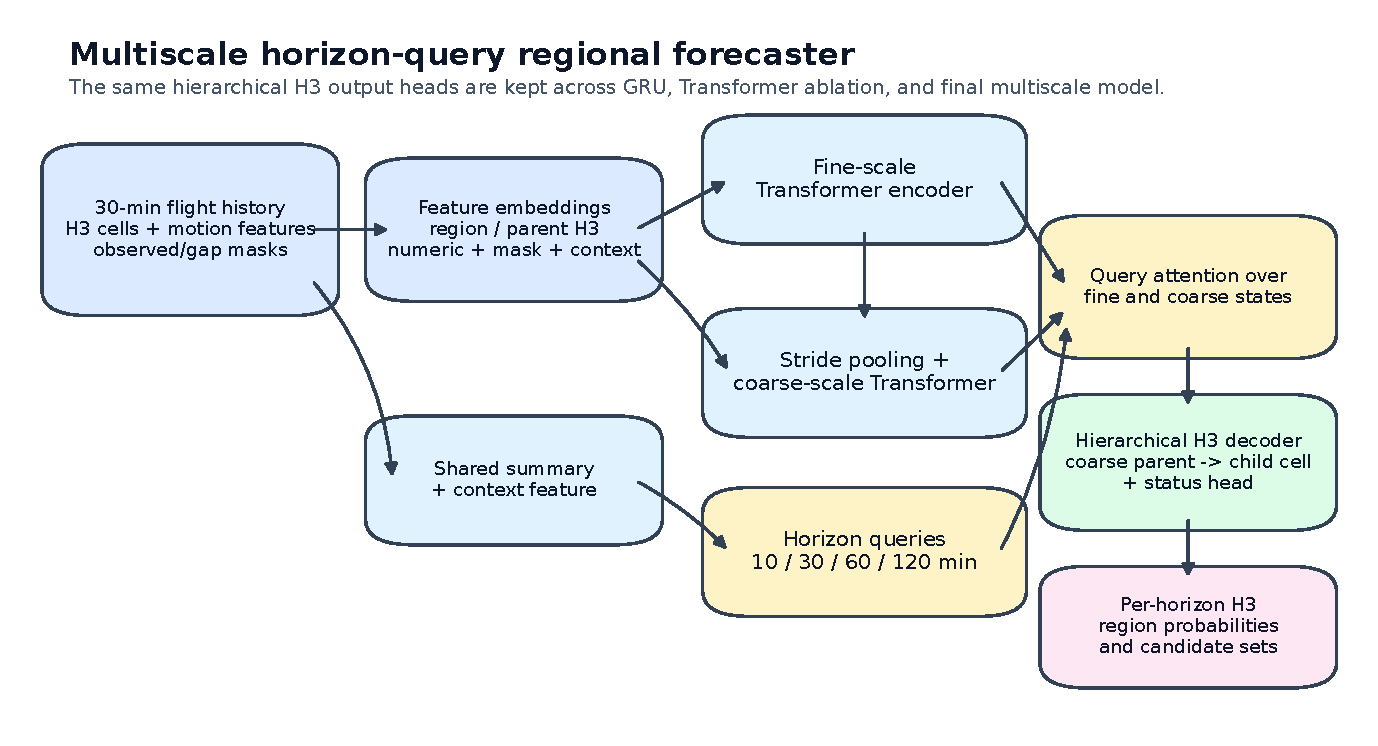
\includegraphics[width=\textwidth]{figures/fig1_method_architecture.pdf}
\caption{Horizon-Router 方法总览。历史轨迹和轻量上下文首先被编码为 H3/父层 token 与数值特征；多尺度 horizon-query 编码器为每个预测时域检索细尺度和粗尺度历史证据；global、coarse-stable 和 local-causal 三个 expert 经 horizon-level router 融合后，进入 coarse、status 和 child heads，输出层级 H3 区域概率。}
\label{fig:method-architecture-zh}
\end{figure}

\subsection{输入表示与层级 H3 输出}

对每个历史时间步 $z_t=(r_t,p_t,u_t,m_t)$，模型分别学习输入区域 embedding、父层区域 embedding，并将数值特征和 mask 特征线性投影到同一隐空间：
\begin{equation}
\tilde{z}_t = [E_r(r_t); E_p(p_t); W_u u_t; W_m m_t].
\end{equation}
其中 $r_t$ 是输入分辨率 H3 cell，$p_t$ 是其父层 cell，$u_t$ 包含位置、位移、高度、速度、航向、时间间隔等数值特征，$m_t$ 包含 \texttt{observed\_flag} 与 \texttt{gap\_flag}。模型根据观测标记、缺口标记和 unknown token 构造时间有效掩码；该掩码被 Transformer attention、池化和局部编码模块共享，用于抑制填充片段和缺口补齐片段的影响。样本级上下文 $c$ 经过单独线性层投影后参与后续编码。

对每个预测时域 $h_j$，层级输出头预测粗区域、状态和条件子区域：
\begin{equation}
p(y_j^{(c)}, y_j^{(f)}, s_j \mid X,c,h_j)
=
p(s_j \mid X,c,h_j)
p(y_j^{(c)} \mid X,c,h_j)
p(y_j^{(f)} \mid y_j^{(c)},X,c,h_j).
\end{equation}
训练时，子区域交叉熵使用真值粗区域标签作为条件，以稳定学习父子层级对应关系。推理时，模型从粗区域分布中选取 top-$K_j$ 个父区域，再计算每个父区域下的条件子分布，并将父层概率质量散射到细粒度 H3 cell。本文完整实验中使用的父层 top-$K$ 为 $[64,48,48,12]$。

\subsection{多尺度 Horizon-Query 编码器}

单一历史摘要难以同时服务 10 分钟和 120 分钟预测。本文先用带有效掩码的 Transformer encoder 得到细尺度历史序列
\begin{equation}
H^{(f)}=\mathrm{Enc}(W_z\tilde{Z}+P),
\end{equation}
并通过 masked mean pooling 与上下文投影拼接为共享基特征 $b$。随后，模型按 stride $=2$ 对 $H^{(f)}$ 做带掩码的局部均值池化，再经一个粗尺度 Transformer encoder 得到
\begin{equation}
H^{(c)} = \mathrm{Enc}_{c}(\mathrm{Pool}(H^{(f)})).
\end{equation}

对每个 horizon，模型维护可学习 horizon embedding $e_j$，并构造时域查询向量
\begin{equation}
q_j = W_q[b;e_j].
\end{equation}
该查询分别对细尺度序列和粗尺度序列做交叉注意力：
\begin{equation}
\alpha_j^{(f)}=\mathrm{softmax}(q_j {H^{(f)}}^\top),\qquad
\alpha_j^{(c)}=\mathrm{softmax}(q_j {H^{(c)}}^\top),
\end{equation}
\begin{equation}
z_j^{(f)}=\alpha_j^{(f)}H^{(f)},\qquad
z_j^{(c)}=\alpha_j^{(c)}H^{(c)}.
\end{equation}
多尺度 horizon-query 特征写为
\begin{equation}
g_j=\phi_g([b;z_j^{(f)};z_j^{(c)};e_j]).
\end{equation}
这里的 $g_j$ 同时也是 Horizon-Router 中的 global expert：它保留完整历史、细尺度注意力和粗尺度注意力，是 warm-start 时最强的单路径预测分支。

\subsection{Horizon-Router 三专家融合}

Horizon-Router 在 global expert 之外加入两个分工明确的 expert。coarse-stable expert 只依赖粗尺度序列摘要和粗尺度注意力：
\begin{equation}
c_j=\phi_c([b^{(c)};z_j^{(c)};e_j]),
\end{equation}
其中 $b^{(c)}$ 是粗尺度序列的 masked mean pooling 与上下文投影拼接。该分支强调阶段性趋势和粗粒度稳定演化，主要服务中长时域预测。

local-causal expert 只读取最近若干历史步，并使用因果 Transformer encoder 抑制对未来位置的泄漏。设最近局部序列为 $H^{(\ell)}$，则短时 horizon 的局部特征为
\begin{equation}
\ell_j=\phi_\ell([b;z_j^{(\ell)};e_j]),\qquad
z_j^{(\ell)}=\mathrm{Attn}(q_j,H^{(\ell)}).
\end{equation}
在实现中，local-causal expert 只对预设的短时 horizon 激活；对更长 horizon，该分支通过 active expert mask 被置为不可用。这个边界很重要：局部机动对 10 或 30 分钟预测有价值，但不应被强行解释为 120 分钟区域需求的主证据。

router 在每个 horizon 上读取三个 expert 特征和 horizon embedding，输出融合权重：
\begin{equation}
w_j=\mathrm{softmax}(R([g_j;c_j;\ell_j;e_j]))\in\mathbb{R}^3.
\end{equation}
最终解码特征为
\begin{equation}
d_j=w_{j,g}g_j+w_{j,c}c_j+w_{j,\ell}\ell_j.
\end{equation}
$d_j$ 被送入共享的粗区域头、状态头和条件子区域头。与简单加深单一路径编码器相比，这一结构让模型可以在时域层面选择历史证据来源，而不必要求所有 horizon 使用同一种时间摘要。

\subsection{训练目标与路由约束}

基础层级损失由粗区域、子区域和状态交叉熵组成。设 $\mathcal{V}$ 为 batch 中有效 horizon 集合，则
\begin{equation}
\mathcal{L}_{\text{hier}}
=
\frac{1}{|\mathcal{V}|}
\sum_{j\in\mathcal{V}}
\left(
\mathcal{L}^{(j)}_{\text{coarse}}
+
\mathcal{L}^{(j)}_{\text{child}}
+
\mathcal{L}^{(j)}_{\text{status}}
\right).
\end{equation}

为了避免 router 过早偏向单一 expert，本文加入 loss-aware router supervision。对每个有效 horizon 和每个 active expert，模型临时用该 expert 特征通过共享输出头计算 expert loss $L_{j,e}$，并构造 soft target：
\begin{equation}
\hat{w}_{j,e}=
\frac{\exp(-L_{j,e}/\tau)}
{\sum_{e'\in\mathcal{A}_j}\exp(-L_{j,e'}/\tau)}.
\end{equation}
其中 $\mathcal{A}_j$ 是 horizon $j$ 上的 active expert 集合，$\tau$ 是 router supervision temperature。router supervision 最小化 $\hat{w}_j$ 与 $w_j$ 之间的 KL 散度。active expert mask 用于屏蔽长时域上的 local-causal expert，避免该分支在不适用的 horizon 上接受错误激励。

本文还加入两个轻量约束。load balancing loss 将 router 权重拉向 active expert 上的均匀分布，防止单个 expert 长期占用全部概率质量；expert auxiliary loss 对 coarse-stable 和可用的 local-causal 分支施加输出头辅助监督，使这些分支即便未被 router 频繁选择也能保持可训练。global expert 通过主输出路径接受监督。

最后，模型使用 horizon-wise teacher distillation 稳定概率输出。训练时，从若干与层级输出兼容的强神经专家中按 horizon 构造混合教师分布，并对学生模型的 coarse、child 和 status 概率施加 KL 蒸馏项。总目标可写为
\begin{equation}
\mathcal{L}
=
\mathcal{L}_{\text{hier}}
+
\lambda_{\text{route}}\mathcal{L}_{\text{route}}
+
\lambda_{\text{bal}}\mathcal{L}_{\text{bal}}
+
\lambda_{\text{aux}}\mathcal{L}_{\text{aux}}
+
\lambda_{\text{distill}}\mathcal{L}_{\text{distill}}.
\end{equation}
完整实验使用的权重为：$\lambda_{\text{distill}}=0.08$，状态蒸馏权重 $0.01$，$\lambda_{\text{route}}=0.08$，$\lambda_{\text{bal}}=0.02$，$\lambda_{\text{aux}}=0.05$，router supervision temperature 为 $0.7$。

\subsection{推理概率支撑}

推理阶段，模型先从粗区域分布中保留每个 horizon 的 top-$K_j$ 父区域，再在这些父区域下展开条件子区域概率，并将父层概率质量散射回细粒度 H3 cell。为避免将概率分配给明显超出运动学范围的区域，本文在所有模型上使用相同的可达性掩码。该掩码根据当前 H3 cell 中心到目标 cell 中心的球面距离构造；若某目标 cell 的距离超过
\begin{equation}
d_{\max}(h_j)
=
v_{\max}\cdot 1.852 \cdot \frac{h_j}{60}
+
\Delta,
\end{equation}
则其概率被置零并重新归一化。本文默认采用 $v_{\max}=750$ knots、$\Delta=250$ km。该步骤只作为统一推理约束，不参与训练，也不作为 Horizon-Router 的方法贡献。

\section{实验设置}

\subsection{数据与划分协议}

实验使用基于 ADRR 构建的 2024 年 3 月商业航班轨迹档案。按照项目既有流程，原始记录先按 90 分钟时间缺口切分为 mission，并对不超过 30 分钟的局部缺口做规则化处理；随后轨迹被重采样到 5 分钟时间网格，并构造区域、数值、mask 和上下文特征。为避免过短或信息不足的片段进入训练集，本文要求有效轨迹段至少包含 8 个重采样点。

处理完成后，数据集中共有 20,712,602 个预测窗口，其中训练集、验证集和测试集分别包含 14,505,637、3,108,933 和 3,098,032 个窗口。与很多窗口级随机切分方案不同，本文按航空器 id 进行 train/val/test 划分，从而尽量避免同一航空器的重复运行模式同时出现在训练和测试中。由于研究对象是开放运行档案而非单机场局部场景，这样的划分更接近真实部署时面对未见航空器或未见轨迹片段的情形。

\subsection{时间与空间协议}

所有模型统一使用 30 分钟历史、5 分钟采样间隔和 4 个预测时域 $\{10,30,60,120\}$ 分钟。对应的输入历史长度为 6 个时间步。空间离散化基于 H3：输入区域分辨率为 3，其父层输入分辨率为 2；目标细粒度分辨率为 $[3,3,2,2]$，对应粗粒度分辨率为 $[2,2,1,1]$。这一设置意味着 10 和 30 分钟预测仍保留较细空间粒度，而 60 和 120 分钟预测则在更宽的空间支撑上建模未来不确定性。

在层级推理阶段，粗区域 top-$K$ 值统一设置为 $[64,48,48,12]$。该设置兼顾了短时域更大的局部候选分支和长时域更粗空间分辨率下较小的父层类别规模。

\subsection{比较模型}

本文报告六类代表性模型。
\begin{enumerate}
  \item \textbf{Markov baseline}：以当前输入区域为状态，统计从当前区域到未来区域和未来状态的经验转移频次，并使用加一平滑得到各 horizon 上的区域和状态概率。
  \item \textbf{Hierarchical GRU}：项目原始层级区域预测基线，使用共享 GRU 时间摘要和 coarse-to-fine H3 输出头。
  \item \textbf{Transformer Horizon Decoder}：在层级 H3 输出头不变的条件下，用单尺度 horizon-query Transformer 替代 GRU 共享时间摘要。
  \item \textbf{Multiscale Transformer}：本文提出的最终模型，在单尺度 horizon-query 基础上加入显式粗尺度时间分支。
  \item \textbf{TrAISformer-H3}：保留 TrAISformer 风格的因果离散序列建模结构，并将其输出端适配为本文统一的层级 H3 输出头。
  \item \textbf{FlightBERT++-H3}：保留 FlightBERT++ 风格的非自回归 encoder-decoder 多 horizon 解码结构，并将原始飞行状态输出替换为本文统一的层级 H3 输出头。
\end{enumerate}

这里的 TrAISformer-H3 和 FlightBERT++-H3 都是\emph{适配基线}而非原论文任务的逐字复现。为了保证比较公平，我们固定了输入历史、预测时域、H3 输出空间、层级损失和评价指标，只允许时间建模主干和与之相关的训练超参数发生变化。相比之下，大量已有航空轨迹文献仍以短时坐标误差或局部空域点预测为中心，若不经过这一适配过程，无法直接与本文的区域概率预测协议进行同表比较。

\subsection{训练设置与公平性说明}

所有神经模型均在单张 CUDA GPU 上训练，使用 AdamW 优化器和固定随机种子 42。GRU 基线沿用项目原始 full 配置：batch size 为 1024，最大 epoch 为 400，最少训练 15 个 epoch，学习率调度阈值与早停阈值均为 $5\times10^{-4}$。Transformer 家族模型（单尺度 ablation 和最终多尺度模型）统一采用 batch size 1024、8 个 DataLoader workers、混合精度训练、学习率 $1.5\times10^{-4}$、weight decay $10^{-4}$、梯度裁剪 1.0，并使用以下调度和早停配置：最大 epoch 1000、最少训练 8 个 epoch、ReduceLROnPlateau patience 4、factor 0.5、绝对阈值 $3\times10^{-4}$、early stopping patience 8、min delta $3\times10^{-4}$。

对外部适配基线，我们保持相同的数据协议、输出头和评价协议，但允许采用各自稳定收敛所需的吞吐配置。具体而言，TrAISformer-H3 和 FlightBERT++-H3 使用 batch size 2048、12 个 workers、混合精度、学习率 $2\times10^{-4}$，其余调度器和早停规则与 Transformer 家族模型保持一致。这样做的目的不是给予外部基线额外优势，而是避免把它们限制在明显次优的系统吞吐配置上。

最终 full-scale 训练的最佳验证损失和停止轮数分别为：Hierarchical GRU 不再以本文新协议重新调参；Transformer horizon decoder 在第 182 个 epoch 达到最优验证损失 0.3177；最终多尺度模型在第 182 个 epoch 达到最优验证损失 0.3055；TrAISformer-H3 在第 136 个 epoch 达到最优验证损失 0.3077；FlightBERT++-H3 在第 100 个 epoch 达到最优验证损失 0.3149。

\subsection{评价指标}

本文同时从分类性能、概率质量和候选区域效率三个层面评价模型。

\textbf{分类性能。}
我们报告每个 horizon 上的 region top-1/top-3/top-5 命中率，并在主表中给出四个 horizon 的宏平均结果。状态预测同时输出 airborne/landed 概率，但在完整数据集上所有神经模型和 Markov 基线的状态准确率均接近 1.0，因此状态指标只保留为完整性报告，不作为区分模型优劣的主依据。

\textbf{概率质量。}
区域概率通过 NLL、Brier 分数和 10-bin ECE 评价。对层级模型，评价时使用由粗区域分布与条件子区域分布组合得到的细粒度 H3 概率；若真值 coarse 和 child 标签都可用，则 NLL 还可精确写成真值粗区域概率与真值子区域条件概率的乘积形式。

\textbf{候选区域效率。}
对每个 horizon，首先按概率从高到低选取细粒度 cell，直到累计概率质量达到 0.8 或达到 cell 预算 $B=[24,18,18,24]$；再按 H3 1-ring 邻接关系把这些 cell 合并为连通组件，并按组件置信度排序。基于这一构造，本文报告：
\begin{enumerate}
  \item \emph{candidate union cover}（候选并集覆盖率）：真实目标 cell 是否落在全部候选组件并集中；
  \item \emph{candidate union cell count mean} 与 \emph{candidate union area mean}：候选并集的平均规模与平均面积；
  \item \emph{Cover@Budget}（固定预算覆盖率）：只保留固定 cell 预算 $B_j$ 个最高概率 cell 时的覆盖率；
  \item \emph{Area@Budget}：对应固定 cell 预算下的平均区域面积。
\end{enumerate}
其中，候选并集覆盖率回答的是“在给定概率质量预算下，候选并集能否覆盖真实未来位置”；固定预算覆盖率则更直接反映固定空间预算下的召回能力。

\subsection{默认后处理与消融设置}

除非特别说明，主结果默认启用 reachability filter，不启用 H3 neighbor refinement。Reachability filter 根据当前 H3 cell 到目标 H3 cell 的球面距离剔除明显不可达的区域，阈值由最大速度 750 knots 和额外 250 km 余量共同决定。H3 refinement 则只在消融实验中使用，统一采用 1-ring 邻域，并测试 $\alpha\in\{0.05,0.10,0.20\}$ 三个概率扩散强度。此外，本文还单独报告关闭 reachability filter 的评价结果，以区分“模型本身的概率分布”与“几何可达性约束”对最终指标的贡献。

\section{结果}

\subsection{完整规模主结果比较}

表~\ref{tab:main-results-zh} 报告四个预测时域上的宏平均结果。

\begin{table}[!t]
\centering
\small
\resizebox{\textwidth}{!}{%
\begin{tabular}{lcccccccccc}
\toprule
模型 & Top1 & Top3 & Top5 & NLL & Brier & ECE & Union Cover & Union Cells & Union Area km$^2$ & Cover@Budget \\
\midrule
Markov 基线 & 0.3184 & 0.6166 & 0.7587 & 2.2788 & 0.8111 & 0.0323 & 0.8749 & 9.9542 & 545174 & 0.9699 \\
层级 GRU & 0.6648 & 0.9076 & 0.9631 & 1.0214 & 0.4578 & 0.0180 & 0.8931 & 2.4189 & 128965 & 0.9980 \\
TrAISformer-H3 & 0.6803 & \textbf{0.9178} & \textbf{0.9697} & \textbf{0.9556} & 0.4361 & 0.0094 & \textbf{0.8939} & 2.2297 & 122810 & \textbf{0.9983} \\
FlightBERT++-H3 & 0.6764 & 0.9144 & 0.9671 & 0.9791 & 0.4417 & \textbf{0.0086} & 0.8883 & 2.2023 & \textbf{117593} & 0.9982 \\
Transformer horizon decoder & 0.6744 & 0.9129 & 0.9656 & 0.9946 & 0.4447 & 0.0123 & 0.8920 & 2.2721 & 122553 & 0.9981 \\
\textbf{所提出的多尺度模型} & \textbf{0.6827} & 0.9174 & 0.9685 & 0.9641 & \textbf{0.4338} & 0.0093 & 0.8922 & \textbf{2.1829} & 118810 & 0.9983 \\
\bottomrule
\end{tabular}

}
\caption{10、30、60 和 120 分钟预测时域上的完整规模宏平均比较。}
\label{tab:main-results-zh}
\end{table}

\begin{figure}[!t]
\centering
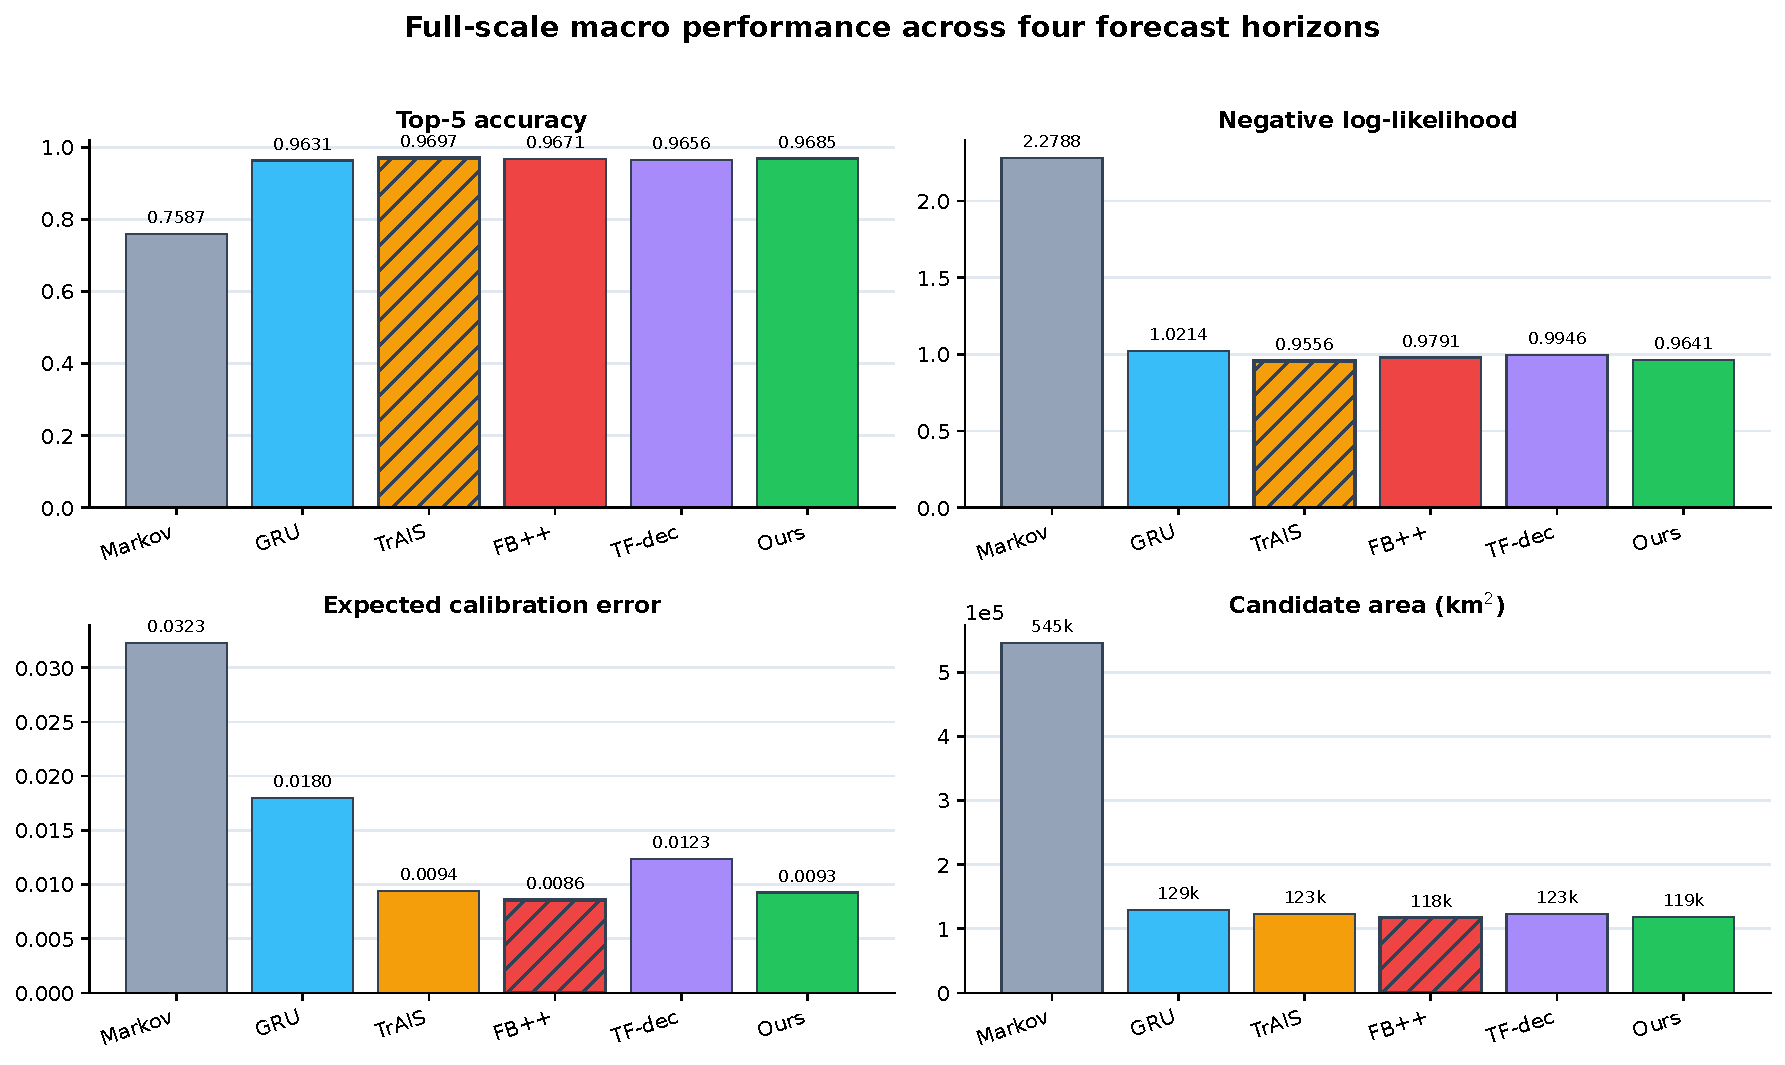
\includegraphics[width=\textwidth]{figures/fig2_main_results_overview.pdf}
\caption{完整规模主结果概览。相较内部基线和两个外部适配基线，所提出的多尺度模型在 top-1、Brier 分数和候选集合紧致性上保持整体最优平衡。}
\label{fig:main-results-overview-zh}
\end{figure}

结果有三点值得注意。首先，所有学习型层级模型都显著优于经典 Markov 基线。其次，在两个外部适配基线中，TrAISformer-H3 是最强竞争者：它取得最高的宏平均 top-3/top-5、最低的 NLL，以及最高的 union cover。第三，所提出的多尺度模型仍然保持最佳宏平均 top-1（0.6827）、最佳 Brier 分数（0.4338）和最小的 candidate union cell 数（2.1829），说明它在分类正确性、概率质量和候选集合紧致性之间取得了更均衡的折中。

FlightBERT++-H3 呈现另一种行为模式。它的宏平均 ECE 最低（0.0086），候选 union 面积也最小（117,593 km$^2$），但 top-1/top-3/top-5 和 union cover 均低于所提模型。这说明更保守、更紧的候选集合并不自动意味着更好的整体区域预测；如果排序能力下降，候选覆盖也会同步退化。

从逐时域结果看，TrAISformer-H3 在 10 和 30 分钟时域上略优于所提模型的 top-3/top-5，但在 120 分钟时域上，所提模型重新取得明显优势：top-1 从 0.5481 提升到 0.5565，top-3 从 0.8482 提升到 0.8531，top-5 从 0.9355 提升到 0.9372，同时 NLL、Brier 和 ECE 也全部更优。这一现象支持本文的核心判断：显式多尺度时间建模的价值主要体现在中长时域区域预测，而不是只在短时排序指标上获益。

\subsection{相较层级 GRU 基线的提升}

相较层级 GRU 基线，所提模型提升了所有 top-k 指标和所有概率指标：top-1 从 0.6648 提升到 0.6827，top-3 从 0.9076 提升到 0.9174，top-5 从 0.9631 提升到 0.9685；NLL 从 1.0214 降至 0.9641，Brier 分数从 0.4578 降至 0.4338，ECE 从 0.0180 降至 0.0093。

提升在不同预测时域上具有一致性。表~\ref{tab:delta-gru-zh} 给出了相较 GRU 基线的逐时域差值。

\begin{table}[!t]
\centering
\small
\resizebox{\textwidth}{!}{%
\begin{tabular}{cccccccccc}
\toprule
时域 & $\Delta$Top1 & $\Delta$Top3 & $\Delta$Top5 & $\Delta$NLL & $\Delta$Brier & $\Delta$ECE & $\Delta$Union Cover & $\Delta$Union Cells & $\Delta$Union Area km$^2$ \\
\midrule
10m & +0.0199 & +0.0059 & +0.0031 & -0.0516 & -0.0281 & -0.0085 & -0.0004 & -0.1864 & -2316 \\
30m & +0.0214 & +0.0129 & +0.0076 & -0.0759 & -0.0303 & -0.0210 & -0.0052 & -0.3683 & -4567 \\
60m & +0.0115 & +0.0054 & +0.0018 & -0.0340 & -0.0158 & -0.0016 & +0.0023 & -0.0908 & -7705 \\
120m & +0.0190 & +0.0153 & +0.0091 & -0.0674 & -0.0220 & -0.0040 & -0.0005 & -0.2988 & -26031 \\
\bottomrule
\end{tabular}

}
\caption{所提模型相较层级 GRU 基线的逐时域差值。对于 top-k 和 union cover，正值更好；对于 NLL、Brier、ECE、候选 cell 和候选面积，负值更好。}
\label{tab:delta-gru-zh}
\end{table}

\subsection{结构消融：多尺度分支是否必要}

为了分离显式多尺度时间编码的价值，我们将最终模型与单尺度 Transformer horizon decoder 比较。后者已经具有时域专属 query，但不包含多尺度分支。

\begin{table}[!t]
\centering
\small
\resizebox{\textwidth}{!}{%
\begin{tabular}{lccccc}
\toprule
模型 & Top1 & Top5 & NLL & Brier & ECE \\
\midrule
Transformer horizon decoder & 0.6744 & 0.9656 & 0.9946 & 0.4447 & 0.0123 \\
Multiscale Transformer & 0.6827 & 0.9685 & 0.9641 & 0.4338 & \textbf{0.0093} \\
\textbf{Horizon-Router} & \textbf{0.6884} & \textbf{0.9710} & \textbf{0.9399} & \textbf{0.4262} & 0.0104 \\
\bottomrule
\end{tabular}

}
\caption{单尺度 Transformer horizon decoder 与所提出多尺度模型的结构消融比较。}
\label{tab:structural-ablation-zh}
\end{table}

多尺度分支改善了所有主要宏平均指标，并取得更低的验证损失（0.3055 对 0.3177）。这支持本文判断：显式双尺度时间建模带来的收益，并不只是把 GRU 替换为 Transformer 所能解释。

\subsection{H3 邻域 refinement 体现召回与校准的权衡}

接着，我们在三个扩散强度上评估 H3 邻域 refinement。该策略提高了概率质量候选召回，但不是无代价收益。

\begin{table}[!t]
\centering
\small
\resizebox{\textwidth}{!}{%
\begin{tabular}{lcccccccc}
\toprule
模型 & Top5 & NLL & Brier & ECE & Union Cover & Union Cells & Union Area km$^2$ & Cover@Budget \\
\midrule
最终模型 & 0.9685 & 0.9641 & 0.4338 & 0.0093 & 0.8922 & 2.1829 & 118810 & 0.9983 \\
Refine a=0.05 & 0.9677 & 0.9593 & 0.4344 & 0.0310 & 0.9052 & 2.3315 & 127062 & 0.9987 \\
Refine a=0.10 & 0.9673 & 0.9796 & 0.4372 & 0.0585 & 0.9192 & 2.5168 & 137220 & 0.9987 \\
Refine a=0.20 & 0.9662 & 1.0340 & 0.4493 & 0.1135 & 0.9496 & 3.0980 & 167889 & 0.9987 \\
\bottomrule
\end{tabular}

}
\caption{完整数据集上的 H3 邻域 refinement sweep。更高的 union cover 伴随更差的校准性和更大的候选集合。}
\label{tab:h3-refine-zh}
\end{table}

\begin{figure}[!t]
\centering
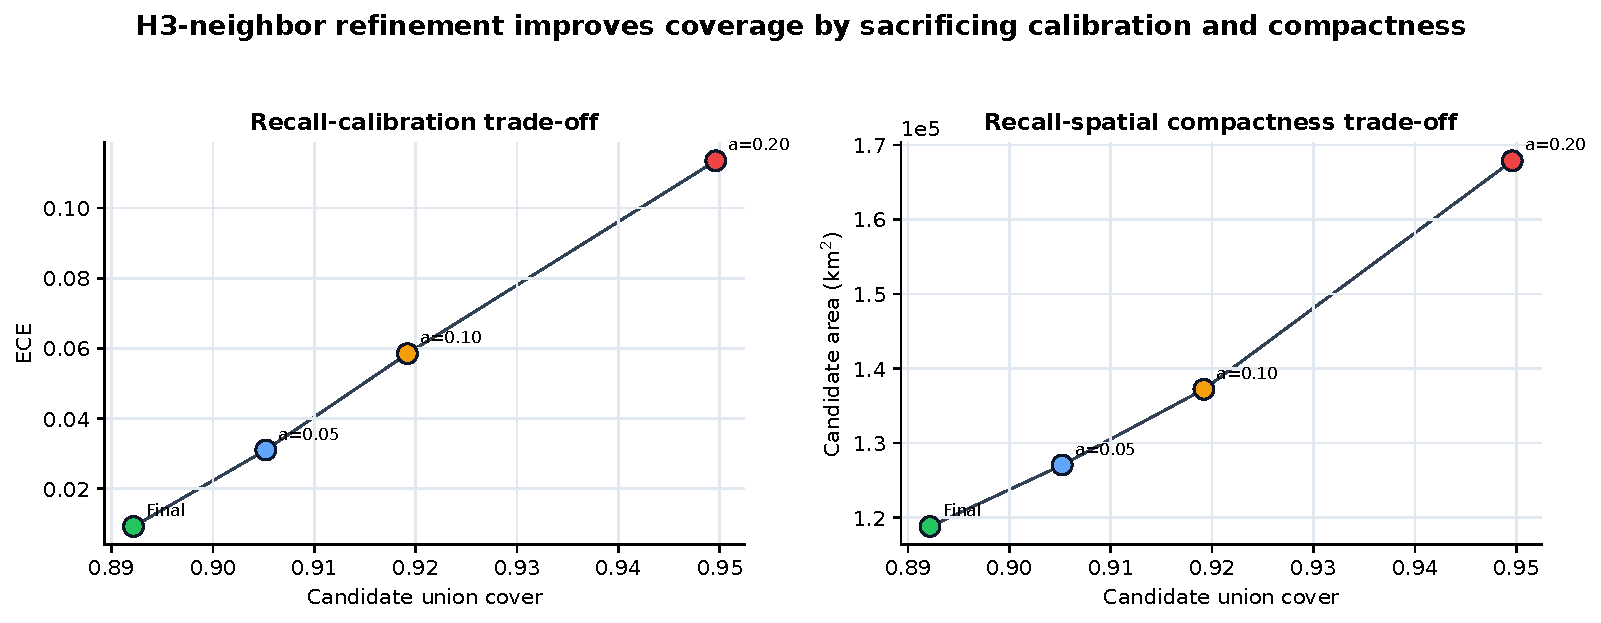
\includegraphics[width=0.78\textwidth]{figures/fig3_h3_refinement_tradeoff.pdf}
\caption{H3 邻域 refinement 提高候选 union cover，但额外召回以更差校准性和更大空间候选面积为代价。}
\label{fig:h3-refinement-tradeoff-zh}
\end{figure}

refinement 提高了候选 union cover，但很快损害校准性，并最终恶化 top-5 和 NLL。因此，它不应作为最终模型呈现。它的价值在于揭示一个具有运行意义的权衡：本地空间平滑可以提高召回，但会牺牲置信度质量和空间紧凑性。

\subsection{Reachability filtering 的聚合影响较小}

关闭 reachability filtering 只带来很小的聚合指标变化。这说明在当前设置中，reachability filtering 更像是一个可达性合理性保护，而不是预测收益的主要来源。

\section{讨论与限制}

本文的主要结果不是简单证明 Transformer 优于 GRU，而是说明多时域区域航空预测需要两层时域适配。第一层是多尺度 horizon-query 编码：不同预测提前量应分别读取细尺度和粗尺度历史证据。第二层是 Horizon-Router：当短时局部机动、粗尺度稳定趋势和完整历史多尺度趋势同时存在时，时域级 router 可以为不同 horizon 选择更合适的 expert 组合。

区域化表述本身也很重要。在开放运行数据上，尤其是 60 到 120 分钟预测时域，长距离点式轨迹回归容易制造并不可靠的精确感。H3 区域概率把不确定性显式化，使 top-$k$ 排序、NLL、Brier 和 ECE 能够在同一离散概率空间中比较。本文本轮主结果刻意不报告预测集合面积，以免把额外集合构造与模型概率质量混在一起；预测集合大小、空间面积和覆盖风险之间的关系需要在后续用更独立的协议评价。

当前论文也有明确边界。首先，虽然 H3 表示在空间上是通用的，但本文实验使用的是 ADRR 中一个月商业航班运行档案，不应被解读为已经覆盖所有航空运行场景。更广泛的跨区域、跨季节和跨数据源验证仍然需要后续实验。

其次，当前模型保留 gap indicator，但没有显式建模缺失观测造成的不确定性。模型也不是 GRU-D、连续时间潜变量动力学或 conformal regional prediction 意义上的缺失感知预测器。这一部分应作为下一阶段工作，而不是当前论文的隐含贡献。

第三，路由训练机制仍需要完整规模逐项消融。当前 full-scale 证据主要体现在最终 Horizon-Router 相较 Multiscale Transformer 的提升；若要把 horizon-wise distillation、router supervision、load balancing 和 expert auxiliary loss 分别作为强因果贡献，还需要在相同数据划分和训练预算下补齐 router only、router + horizon-wise distillation、router + horizon-wise distillation + loss-aware routing regularization 三组实验。

最后，外部航空基线受任务不匹配限制较大。现有许多文献处理短时坐标预测、终端区交互，或依赖当前 ADRR 派生 artifact 中不可用的密集上下文输入。本文因此采用适配后的 TrAISformer-H3 和 FlightBERT++-H3 作为强基线，并明确固定数据、输出头和评价协议。该选择保证了同表比较的可解释性，但也意味着本文不是对原论文任务的逐字复现。

\section{结论}

本文基于 ADRR 派生开放航空数据，对多时域区域航空轨迹预测进行了大规模实验研究。以层级 H3 GRU 基线为起点，我们引入 horizon-query Transformer decoder，并进一步加入显式多尺度时间分支。最终模型相较 GRU 基线和单尺度 Transformer 消融模型，在 top-k 准确率、NLL、Brier 分数和校准性上均取得提升，同时生成更小的候选区域集合。经典 Markov 基线明显较弱，这说明该任务需要比简单经验转移建模更强的时间表示学习能力。

H3 refinement 实验进一步说明，候选召回和校准性应当一起报告。一个激进扩展候选区域的模型，在只看召回时可能显得更强，但其概率可信度会下降。因此，大规模区域航空预测应被评估为准确性、不确定性质量和空间效率的联合问题。

总体而言，实验结果支持将层级 H3 预测与多尺度 horizon-query 时间编码结合，作为开放轨迹档案上长时域区域航空预测的强基线。它也为下一步方法研究提供了稳定基础：在缺失和不规则飞行观测下，进一步构建显式不确定性感知的区域预测模型。

\section*{数据可用性与可复现性}

本文实验使用一个月的飞行轨迹，数据来源于 EUROCONTROL Aviation Data Repository for Research（ADRR）~\cite{eurocontrol_adrr_2025}。EUROCONTROL 按其使用条款向研究和开发用途提供 ADRR 访问，但原始数据不能由本文作者公开再分发。为支持可复现性，项目仓库包含用于标准化 ADRR 数据的端到端预处理脚本、所有报告实验的配置文件、所有比较方法的模型实现、实验日志和评估摘要，以及用于重建开发子集和重新运行完整实验的脚本。


\bibliographystyle{unsrtnat}
\bibliography{paper_refs_v1}
\end{document}
